\documentclass[journal]{IEEEtran}

  \usepackage[pdftex]{graphicx}
  \usepackage[justification=centering]{caption}
  \DeclareGraphicsExtensions{.png}

\hyphenation{op-tical net-works semi-conduc-tor}


\begin{document}

\title{An Infrastructure for Automatic Installation of Applications Based on the User's Context}

\author{
        Leandro M. de Sales,
        Bruno G. Ferreira,
        Durval P. C. Neto,
        Larissa A. L. Monteiro
}

\maketitle

\begin{abstract}
This paper presents a context-aware middleware that performs automatic installation of relevant applications on user’s mobile device based on user current location.
\end{abstract}

\IEEEpeerreviewmaketitle



\section{Introduction}

\IEEEPARstart{W}{ith} the creation of the term Ubiquitous Computing, Mark Weiser envisioned a world where computing was intrinsic to the routine of the population, adding tools to its users, without requiring much effort or technical knowledge.  However, currently, the distribution of applications is centralized in virtual stores, which means users need to access a virtual store, perform a search and finally select the desired application for download. When the download is completed, the user will need to install the application, which requires the authorization of some permissions for the application to access the features of your gadget, like camera, microphone, bluetooth and others. The world idealized by Mark do not exist because it is required much effort of the user to get an application from the store, rather then when the user knows the existence of this application. It is proposed in this paper a way of providing self-installable applications related to a context/environment to users who are in this context/environment, without the need of so much effort. This solution uses the UPnP technology and consists of two modules, the BRisa Central Apps (BCA) and the BRisa Central User (BCU), which will be explained in the Architecture section.

\section{Architecture}
The BCU does the job of the Control Point, searching in all the networks that it is connected for a BCA, who makes the job of the Device and correspond all the BCU's which requires them.  The BCA is installed on a computer located in environments where the applications will be served. The BCU is installed on the mobile device of each user who wishes to receive applications available in the environments.
    The protocol who manage all the communication between the BCA and the BCU is called BRisa Apps Communication Protocol(BACP). This architecture offers peer-to-peer pervasive network connectivity between all types of devices including laptops and desktops. Also, the International Organization for Standardization and the International Electrotechnical Commission considered UPnP as the leading technology for discovery and control of networked devices [4].
The communication process between the BCU and the BCA is summarized in Fig. 1. In Step 1, when the BCU enters on a new environment and connects to the network, it sends a request to discover BCA’s through the UPnP discovery protocol, known as the Simple Service Discovery Protocol (SSDP). In Step 2, upon

\begin{figure}[tb]
    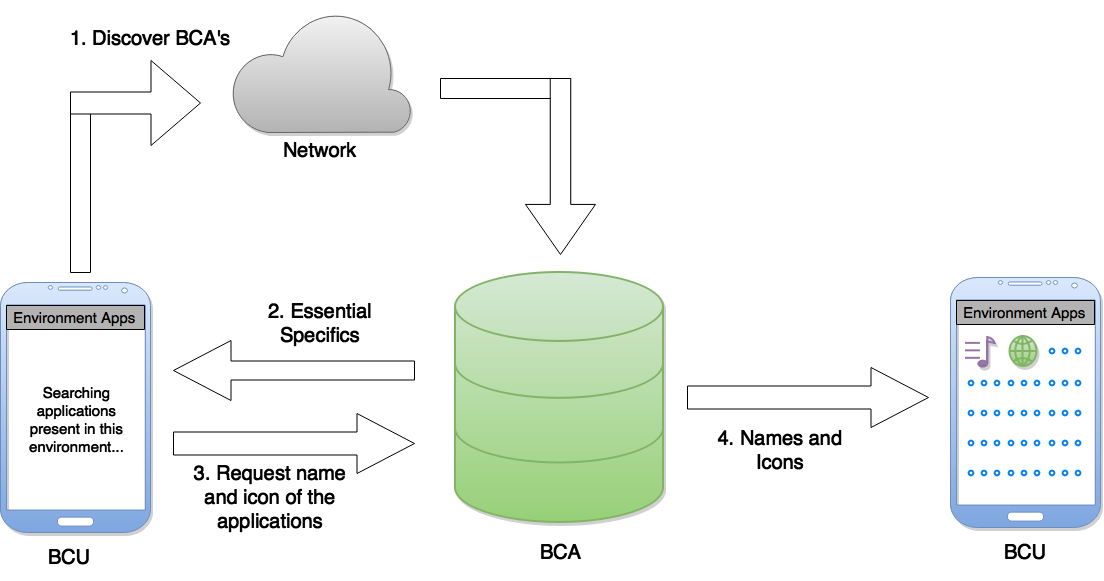
\includegraphics[scale = 0.26]{FIG1}    
    \rule[1ex]{10cm}{0.5pt}
\end{figure}

\begin{figure}[tb]
    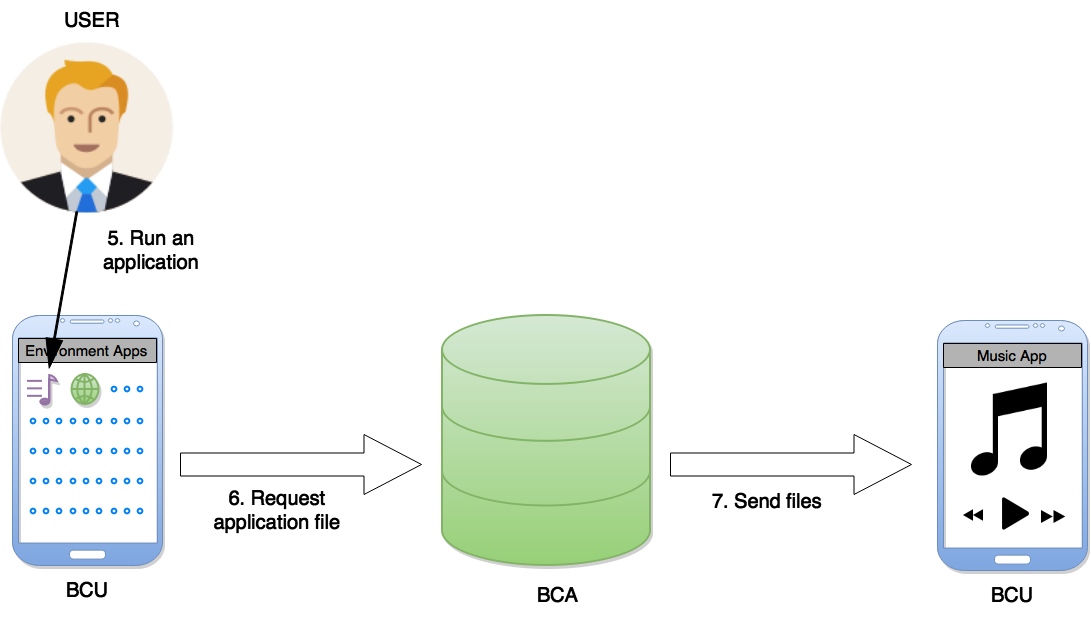
\includegraphics[scale = 0.26]{FIG2}
    \caption{Automatic application installation process.}
\end{figure}

receiving the discover message, the BCA reply to the BCU by sending a message that contains important information about the device and related information about the services for allowing the BCU to install the available applications. In Step 3, the BCU sends a request for each BCA found asking for the name and icon of each application the respective BCA’s are hosting. Once the BCU receives the reply from its BCA (Step 4), each application icon is exposed on the applications menu of the BCU. In Step 5, if the user is interested in any of the applications that appear on the screen, (s)he can “click” on its icon, and then, in Step 6, the BCU sends a request to the respective BCA in order to download the necessary files for loading the selected application. In Step 7, the corresponding files are downloaded in a compressed format and extracted on the BCU. The main application file is then executed and the application is properly loaded. When the user leaves the environment, the application is automatically removed, freeing up storage space on the device.
Optionally, the user can activate a caching mechanism to avoid downloading applications that were previously executed. However, before the client eventually executes the application stored in the cache, the client module checks if a newer version of the application is available in the BCA who host this application. For this, the  BCU executes the BRisa Application Communication Protocol (BACP). A more detailed sequence of requests exchanged by BCU and BCA is depicted in Fig. 2.
In the context of developing application, the Qt/QML language was chosen as the default language for writing applications that will be hosted on the BCA. It is part of the Qt Framework and it is a multi-paradigm language for creating highly dynamic applications.
The format of an application is a set of QML files along with other resources used by the QML files. To host an application on the BCA, the files must be installed in a specific folder present on the BCA. The directory structure of a BCA hosting two applications is depicted in Fig. 3. When the BCA send the list of applications for the BCU, it’s sent a JSON file with the names and the url’s of the icons of the application. When the user choose which application will be executed and click in the icon of the application, the BCA send a JSON with the title, the url of the icon, the a short description and all the services proposed by the application. If the user have been interested by the application, BCA will send a JSON with an url of the main QML of the application or if him have not been interested he can leave it and choose another one.

\section{Description of a Case Study}
Suppose the scenario where a user arrives at a Shopping. The icon of an application provided by the shopping is automatically displayed on the main menu of the BCU. The

\begin{figure}[!htb]
    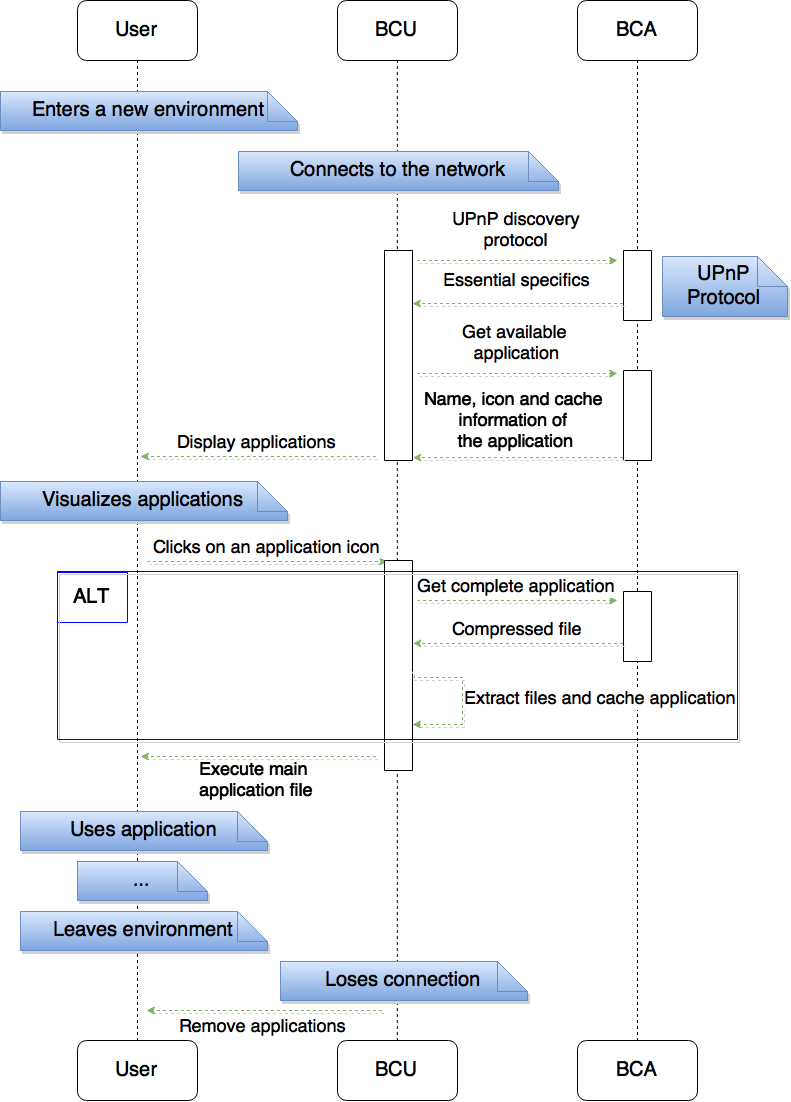
\includegraphics[scale = 0.24]{FIG4}
    \caption{Detailed sequence of requests exchanged by BCU and BCA.}
\end{figure}

\begin{figure}[!htb]
    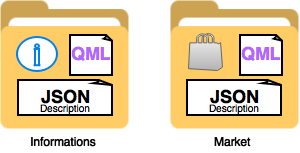
\includegraphics[scale = 0.83]{FIG3}
    \caption{Directory structure of a BCA hosting two applications.}
\end{figure}

main function of the application discussed in this example is to allow users to get information about the stores, buy itens, look for hot sales and other actions. By “clicking” on the icon for loading the just discovered application, the user can perform many actions inside the shopping without the need of walk to the store, or simply move, the only thing (s)he need to do is choose the right application and run it. For example, if the user want to buy a wallet, (s)he looks into the application of the store he want to buy and choose the wallet he wants, them (s)he decides to buy the wallet, from the device (s)he buy and go to the store validate the buy and get the buyed item. this kind of application can reduce the total time that an user will take for perfoming his pretended actions in a mall, therefore, avoid spend more time than necessary. When the user leaves the mall, the application is automatically removed from his/her device.

\section{Conclusion}
The middleware presented in this paper provides a basis for specific types of applications useful in a particular location. The applications are installed in the main menu of the BCU without any intervention and/or boring installation process, promoting the Weiser’s vision of the hidden technology for pervasive scenarios such as food court, book store, shopping mall and hotel, to name a few. Therefore, the proposed middleware can improve the user’s experience on using mobile services, avoiding the traditional process of searching and installing applications manually. In some cases, the user does not even know about the existence of a certain application to use in a given place, therefore, the proposed middleware can be used to expose available services in the environment before hidden for the users for not know their existence.

\ifCLASSOPTIONcaptionsoff
  \newpage
\fi 

\begin{thebibliography}{1}

\bibitem{IEEEhowto:kopka}
M.~Weiser, \emph{The computer for the 21st century.}\hskip 1em plus
  0.5em minus 0.4em\relax Scientific American, vol. 265, no. 3, pp. 94–104, Sep. 1991. 
\bibitem{IEEEhowto:kopka}
M.~Satyanarayanan, \emph{Pervasive Computing: Vision and Challenges.}\hskip 1em plus 0.5em minus 0.4em\relax Personal Communications, IEEE, vol. 8, no. 4, pp. 10–17, Aug 2001.
\bibitem{IEEEhowto:kopka}
L.~de~Sales et al., \emph{BRisa UPnP A/V Framework.}\hskip 1em plus 0.5em minus 0.4em\relax in International Conference on Consumer Electronics, 2008, pp. 1–2. 
\bibitem{IEEEhowto:kopka}
L.~Sherwin, \emph{UPnP Specifications Named International Standard for Device Interoperability for IP-Based Devices}\hskip 1em plus 0.5em minus 0.4em\relax 2009, UPnP Website. 
\bibitem{IEEEhowto:kopka}
R.~F. et al, \emph{Hypertext Transfer Protocol – HTTP/1.1}\hskip 1em plus
  0.5em minus 0.4em\relax RFC 2616, Internet Engineering Task Force, 1999. [Online]. Available: http://www.ietf.org/rfc/rfc2616.txt.

\end{thebibliography}

\end{document}


